%pdflatex -halt-on-error -aux-directory=tmp -output-directory=tmp rapport.tex%

\documentclass{article}
\usepackage{amsmath}
\usepackage[utf8]{inputenc}
\usepackage[T1]{fontenc}
\usepackage{graphicx}
\usepackage{hyperref}
\usepackage[francais]{babel}
\usepackage{listings}
\usepackage{xcolor}

\definecolor{codegreen}{rgb}{0,0.6,0}
\definecolor{codegray}{rgb}{0.5,0.5,0.5}
\definecolor{codepurple}{rgb}{0.58,0,0.82}
\definecolor{backcolour}{rgb}{0.95,0.95,0.92}

\lstdefinestyle{mystyle}{
    language=python,
    backgroundcolor=\color{backcolour},   
    commentstyle=\color{codegreen},
    keywordstyle=\color{magenta},
    numberstyle=\tiny\color{codegray},
    stringstyle=\color{codepurple},
    basicstyle=\ttfamily\footnotesize,
    breakatwhitespace=false,         
    breaklines=true,                 
    captionpos=b,                    
    keepspaces=true,                 
    numbers=left,                    
    numbersep=5pt,                  
    showspaces=false,                
    showstringspaces=false,
    showtabs=false,                  
    tabsize=2
}

\lstset{style=mystyle}

\title{Théorie des langages II}
\author{Wassim SAIDANE}
\date{01/03/2021}

\begin{document}
    \pagenumbering{gobble}
    \maketitle
    \pagenumbering{arabic}
    \section*{Note : }
    Ce cours est ma prise de note du cours de L3 infos de Théorie des langages II de Mamadou Kante
    \section*{Chapitre 0 : Langages rationnels et reconaissables}
    Si $A$ est un ensemble fini, on note $A*$ l'ensemble des mots finis (un mot = séquance de lettre). 
    On appelle $A$ un alphabet et les éléments de $A$ des lettres. \\ 
    On notera $\epsilon : $ le mot vide. \\ 
    On appel $L$ un langage est un sous ensemble de $A*$. \\ 
    Rappel : La concaténation de mots dera notée ".". \\
    Voici les opérations dur les langages : \\ 
    - \underline{Union (notée $\bigcup$) : }\\
    $L \bigcup L'=\{u \in A* \mid u \in L \text{ ou } u \in L'\}$ \\
    - \underline{Produit (notée $.$) ou concaténation : }
    $L . L'=\{uv \in A* \mid u \in L, v \in L'\}$ \\
    - \underline{Itération de Leene (notée $*$) : } \\
    $L*= \bigcup_{i \ge 0} L^{i} \text{ où } L^{0}=\{\epsilon\}$, $L^i=L.L^{i-1} (i \ge 1)$
    - $L^{+}=\bigcup_{i \ge 0} L^{i}$ \\
    \\
    Une expression rationnelle est définie inductivelement : \\ 
    - $\emptyset$ est une expression rationnelle. \\ 
    - a est une expression rationnelle $\forall a \in A$ \\ 
    - Si $r_1$ et $r_2$ sont des expressions rationnellles, alors $r_1+r_2$ et $r_1.r_2$ sont des expressions rationnelles. \\
    - Si $r$ est une expression rationnelle, alors $r*$ l'est aussi. 
    \\
    Si $r$ est une expression rationnelle, alors son langage noté $L(r)$ est défini ainsi : 
    $L(r)=\left\{\begin{array}{ll}
        \phi & \text { si } r=\varnothing \\
        \alpha \{a\} \text { si } r & =a \\
        L\left(r_{1}\right) U L\left(r_{2}\right) & \text { si } r=r_{1}+r_{2} \\
        L\left(r_{1}\right) \cdot L\left(r_{2}\right) & \text { si } r=r_{1} \cdot r_{2} \\
        L(s)^{*} & \text { si } r=s^{*}
        \end{array}\right.$ \\
    Un langage $L$ est dit \textbf{rationnel} s'il existe une expression rationnelle $r$ telle que $L=L(r)$ \\
    \underline{Automate à états finis}
    Un automate (à états finis) est un tuple $(\Sigma,Q,\delta,I,F)$ tel que : \\
    - $\Sigma$ : Alphabet \\
    - $Q$ : Il s'agit d'un ensemble fini appelé ensemble des états. \\ 
    - $I \subseteq Q $ : Ensemble des états initiaux. \\ 
    - $F \subseteq Q $ : Ensemble des états finaux. \\
    - $\delta$ : $Q \times \Sigma \rightarrow 2^Q$ [$2^Q = P(Q) : $ tous les sous-ensembles de Q] \\
    \\
    Un automate $A$=$(\Sigma,Q,\delta,I,F)$ est : \\
    - Déterministe si $\forall q \in Q, a \in \Sigma, \mid \delta(q,a)\mid \le 1$ \\
    - Complet si $\forall q \in Q, a \in \Sigma, \mid \delta(q,a) \mid \ge 1$ \\
    Si un automate n'est pas déterministe, on dit que c'est un \textbf{automate non déterministe}. 
    \\ 
    Une exécution d'un automate $A=(\Sigma,Q,\delta,I,F)$ sur un mot $u=u_1,u_2,...,u_n$ est une séquance $(q_0,q_1,...,q_n)$ d'états telle que : \\
    - $q_0 \in I$ \\
    - $\forall 1 \le i \le n, q_i=\delta(q_{i-1},u_i)$ \\
    \\
    Un mot $u$ est \textbf{reconnu/accepter} par un automate $A=(\Sigma,Q,\delta,I,F)$ s'il existe une exécution $(q_0,q_1,..,q_n)$ de $A$ sur $u=u_1,u_2,...,u_n$ telle que $q_n \in F$. On parlera d'\textbf{exécution acceptante sur $u$ par $A$}. \\
    \\
    Le langage d'un automate $A$, noté $L(A)$, c'est l'ensemble des mots $u$ acceptées par $A$. \\
    Un langage $L$ est dit \textbf{reconnaissable} s'il existe un automate tel que $L=L(A)$. \\
    \\
    \underline{Théorème 0.1 :} \\
    1) Pour tout langage reconnaissabe L, il existe un \underline{automate déterministe $A$} tel que $L=L(A)$. \\
    2) $\forall$ l'alphabet $\Sigma$, Recog($\Sigma^*$)$=$Rat($\Sigma^*$) \\
    Recog = l'ensemble des langages reconaissables \\
    Rat = L'ensemble des langages rationnels. \\
    \\
    \underline{Remarque :} Les deux points du théorème sont constructifs. \\ 
    - Si $A$ est un automate, on peut construire un automate déterministe $A'$ tel que $L(A)=L(A')$. \\
    \underline{Conséquance : } Pour un automate $A$, savoir si $u \in L(A)$ peut se faore en temps : \\ 
    $f(\mid Q \mid)+2^{O(\mid Q \mid)}.\mid u \mid$ \\ 
    $f(\mid Q \mid)$ : Temps pour construire l'automate déterministe. \\
    $2^{O(\mid Q \mid)}$ : Temps pour tester si un mot $u$ est accepté (le nombre d'états $\le 2^{\mid Q \mid}$). \\
    $\mid u \mid$ : Nombre de lettres du mot $u$. \\
    \\ 
    Preuve de la proposition 1 : si $A=(\Sigma, Q, \delta, I, F)$ est un automate, alors on peut construire un automate déterministe $A'=(\Sigma, Q', \delta', \{\%\}, F')$\\
    où $\mid Q' \mid \le 2^{\mid Q \mid}$. \newpage
    Preuve de la proposition 2 : Pour tout automate $A$, on peut construire une expression rationnelle $r$ telle que $L(A)=L(r_{A})$. \\
    Inversement, pour toute expression rationnelle $r$, on peut construire un automate $A_r$ tel que : \\
    $L(A_r)=L(r)$. \\
    Pour passer des expresiions rationelles aux automates, on définis des opérations sur les automates 
    qui correspondent aux opérations sur les expressions rationnelles. \\ 
    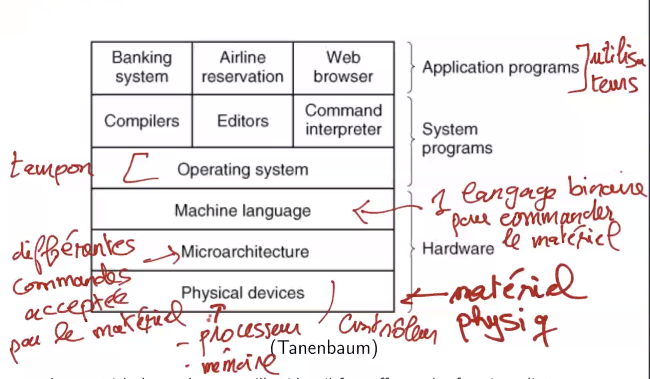
\includegraphics{capture/1.PNG} \\
    \\
    Tous les langages ne sont pas rationels. \\
    Mais, comment montrer qu'un langage n'est pas rationnel ? \\ 
    \underline{Exemple de langage non rationnel : } \\
    - $\{0^n1^n : n \ge 1\}$ \\
    - palindromes \\
    - $\{1^P : p \text{premier}\}$ \\ 
    Pour convaincre, on utilise le lemme de pompage (appelé aussi lemme d'itération). \\
    \\
    \underline{Lemme d'itération des langages rationnels : } Soit $L$ un langage reconaissables. 
    Alors il existe un entier $p$ (appelé \underline{longueur d'itération}) tel que pour tout mot $S$ 
    de taille $\ge p, s$ admet une décomposition en facteurs $x,y,z$ : \\
    1) $s=xyz$ \\
    2) $\mid y \mid > 0$ \\
    3) $\mid xy \mid \le p$ \\
    4) $\forall i \ge 0, xy^iz \in L$ \\
    \\
    \newpage
    \underline{Idée de preuve} \\
    Soit $A=(\Sigma, Q, \delta, I, F)$ un automate reconnaissant $L$. Si un mot $u$ est tel que $\mid u \mid > Q$, $u$ est reconnu par $B$, alors il existera forcément un état $q \in Q$ visite deux fois. 
    Si on regarde l'exécution de $B$ sur $u$. \\
    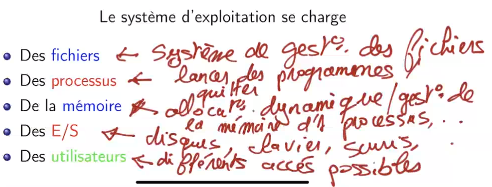
\includegraphics{capture/2.PNG}  \\
    \underline{Exemple d'utilisation} sur $L=\{0^n1^n : n \ge 1\}$ \\
    Preuve par l'absurde : \\
    On va supposer $L$ reconnaissable, notons $p$ la longueur d'itération. On va chercher un mot $w \in L$,
    ensuite on applique le lemme d'itérations sur $w$, on montre ensuite qu'on pourra trouver un mot $w'$, qui est construit
    à partir du lemme d'itération avec $w' \notin L$ et pourtant devrait appartenir à $L$.  \\ 
    \\
    Prenons $w=0^p1^p$. Par le lemme d'itération, $\exists x,y,z$ tel que $w=xyz$, $\mid xy \le p, \mid y \mid \ge 1$ 
    et $\forall i \ge 0, xy'z \in L$. \\
    Comme $\mid xy \mid \supseteq P$, alors $w=0^l0^{l'}0^{l''}1^p$ où $x=0^l$, $y=0^{l'}$, $z=0^l1^p$ $l' \ge 1$. Si on applique la proposition 4
    du lemme d'itération avec $i=0$ on obtient $0^l0^{l''}1^p \in L,$ or $l+l'' < P$. ($l+l'+l''=p, l' \ge 1$) \\
    CONTRADICTION.
\end{document}
